% mnras_template.tex
%
% LaTeX template for creating an MNRAS paper
%
% v3.0 released 14 May 2015
% (version numbers match those of mnras.cls)
%
% Copyright (C) Royal Astronomical Society 2015
% Authors:
% Keith T. Smith (Royal Astronomical Society)

% Change log
%
% v3.0 May 2015
%    Renamed to match the new package name
%    Version number matches mnras.cls
%    A few minor tweaks to wording
% v1.0 September 2013
%    Beta testing only - never publicly released
%    First version: a simple (ish) template for creating an MNRAS paper

%%%%%%%%%%%%%%%%%%%%%%%%%%%%%%%%%%%%%%%%%%%%%%%%%%
% Basic setup. Most papers should leave these options alone.
\documentclass[a4paper,fleqn,usenatbib]{../mnras}

% MNRAS is set in Times font. If you don't have this installed (most LaTeX
% installations will be fine) or prefer the old Computer Modern fonts, comment
% out the following line
\usepackage{newtxtext,newtxmath}
% Depending on your LaTeX fonts installation, you might get better results with one of these:
%\usepackage{mathptmx}
%\usepackage{txfonts}

% Use vector fonts, so it zooms properly in on-screen viewing software
% Don't change these lines unless you know what you are doing
\usepackage[T1]{fontenc}
\usepackage{ae,aecompl}


%%%%% AUTHORS - PLACE YOUR OWN PACKAGES HERE %%%%%

% Only include extra packages if you really need them. Common packages are:
\usepackage{graphicx}	% Including figure files
\usepackage{amsmath}	% Advanced maths commands
\usepackage{amssymb}	% Extra maths symbols

%%%%%%%%%%%%%%%%%%%%%%%%%%%%%%%%%%%%%%%%%%%%%%%%%%

%%%%% AUTHORS - PLACE YOUR OWN COMMANDS HERE %%%%%

% Please keep new commands to a minimum, and use \newcommand not \def to avoid
% overwriting existing commands. Example:
%\newcommand{\pcm}{\,cm$^{-2}$}	% per cm-squared
\newcommand{\Nant}{N_{\text{ant}}} 
\newcommand{\Npix}{N_{\text{pix}}}
\newcommand{\dif}{\mathrm{d}}

%%%%%%%%%%%%%%%%%%%%%%%%%%%%%%%%%%%%%%%%%%%%%%%%%%

%%%%%%%%%%%%%%%%%%% TITLE PAGE %%%%%%%%%%%%%%%%%%%

% Title of the paper, and the short title which is used in the headers.
% Keep the title short and informative.
\title[E-field Parallel Imaging Correlator]{A Generic and Efficient E-field Parallel Imaging Correlator for Next-Generation Radio Telescopes}

% The list of authors, and the short list which is used in the headers.
% If you need two or more lines of authors, add an extra line using \newauthor
\author[Thyagarajan et al.]{
Nithyanandan Thyagarajan,$^{1}$\thanks{E-mail: t\_nithyanandan@asu.edu}
Adam P. Beardsley,$^{1}$
Judd D. Bowman$^{1}$
\newauthor
and Miguel F. Morales$^{2}$
\\
% List of institutions
$^{1}$Arizona State University, School of Earth and Space Exploration, Tempe, AZ 85287, USA\\
$^{2}$University of Washington, Department of Physics, Seattle, WA 98195, USA\\
}

% These dates will be filled out by the publisher
\date{Accepted XXX. Received YYY; in original form ZZZ}

% Enter the current year, for the copyright statements etc.
\pubyear{2015}

% Don't change these lines
\begin{document}
\label{firstpage}
\pagerange{\pageref{firstpage}--\pageref{lastpage}}
\maketitle

% Abstract of the paper
\begin{abstract}
Abstract here (250 words)
\end{abstract}

% Select between one and six entries from the list of approved keywords.
% Don't make up new ones.
\begin{keywords}
instrumentation: interferometers -- techniques: image processing -- techniques: interferometric
\end{keywords}

%%%%%%%%%%%%%%%%%%%%%%%%%%%%%%%%%%%%%%%%%%%%%%%%%%

%%%%%%%%%%%%%%%%% BODY OF PAPER %%%%%%%%%%%%%%%%%%

\section{Introduction}

Radio astronomy is entering an era in which interferometers of hundreds to thousands of individual antennas are needed to achieve desired survey speeds. Nowhere is this more apparent than at radio frequencies below 1.4 GHz. The study of the history of hydrogen gas throughout the universe's evolution is pushing technology development towards arrays of low-cost antennas with large fields of view and densely packed apertures. Similarly, the search for transient objects and regular monitoring of the time-dependent sky is driving instruments in the same direction. A number of new telescopes are under development around the world based on this new paradigm, including the Murchison Widefield Array (MWA, \citealt{tin13}), the Precision Array for Probing the Epoch of Reionization (PAPER, \citealt{par10}), the Hydrogen Epoch of Reionization Array (HERA\footnote{http://reionization.org}), the LOw Frequency ARray (LOFAR, \citealt{dev09}), the Canadian Hydrogen Intensity Mapping Experiment (CHIME, \citealt{ban14}), the Long Wavelength Array (LWA, \citealt{ell13}), and the low frequency component of the Square Kilometer Array Low Frequency Aperture Array (SKA-Low \citealt{mel13}).

This paradigm shift requires a fundamentally new approach to the design of digital correlators \citep{lon00}. Modern correlators calculate the cross-power correlation between all antenna pairs in many narrow frequencies, forming \emph{visibilities}, the traditional fundamental measurement of radio interferometers. The computational requirements for a modern FX correlator scale with the number of antenna pairs, or the square of the number of antennas $\sim \Nant^2$ \citep{bun04}. For this reason traditional correlators have difficulty scaling to thousands of antennas. As an example, the full HERA correlator for 352 dishes with 200 MHz of bandwidth requires 212 trillion complex multiplies and adds per second (TMACS). Future arrays with thousands of collecting elements will require orders of magnitude more computation, making the correlator the dominant cost.

For certain classes of radio arrays there is an alternative to the FX correlator that can lower the computational burden by directly performing a spatial fast Fourier transform (FFT) on the electric fields measured by each antenna in the array at each time step, removing the cross-correlation step. This relieves the computational scaling from the harsh $\Nant^2$ to the more gentle envelope of $\Npix\log\Npix$, where $\Npix$ is the number of pixels in the Fourier transform \citep[e.g.][]{mor11,teg09,teg10}. This architecture is often referred to as a ``direct imaging" correlator because it eliminates the intermediary cross-correlation data products of the FX and earlier lag correlators, but instead directly forms images from the electric field measurements.

Direct imaging correlators have begun to be explored on deployed arrays including the Basic Element for SKA Training II (BEST-2) array \citep{fos14}, the Omniscope \citep{zhe14}, and an earlier incarnation at higher frequencies with the intent of pulsar timing \citep{oto94, dai00}. However, each of these examples make assumptions about the redundancy of the array layout, and require the collecting elements are identical. On the other hand, the MOFF algorithm achieves the same $\Npix \log \Npix$ computational scaling without placing any restriction on antenna placement, can accommodate non-identical beam patterns, and is a provably optimal mapping \citep{mor11}. This algorithm uses the antenna beam patterns to grid the electric field measurements to a regular grid in the software holography/A-transpose fashion \citep{mor09,bha08,teg97b} before performing the spatial FFT. This process has been shown to theoretically produce a data product identical to images produced from the traditional FX correlator.

Here we present the first software implementation of the MOFF correlator, and announce the public release of the E-field Parallel Imaging Correlator (EPIC) code. We begin with a technical description of the algorithm in \S \ref{sec:math}, then discuss our particular implementation in \S \ref{sec:software}. We then verify the output data quality from our code in \S \ref{sec:verify} by presenting simulated images from both the EPIC correlator and comparing to a simulated FX correlator. We also demonstrate the performance with real-world data from the LWA. In \S \ref{sec:analysis} we analyze the scaling relationships of the algorithm. We identify specific array design classes where the EPIC correlator is computationally more efficient than the FX algorithm. We conclude and discuss future research prospects in \S\ref{sec:conclusions}.

% Motivate MOFF from a technical and scientific standpoint. Refer to \citet{del07,mor09,mor11}.

\section{Mathematical Framework}\label{sec:math}

We provide a quick summary of the mathematical equivalence of the MOFF and FX correlators detailed in \citet{mor11}.

Electric fields from astrophysical sources, $E(\hat{\mathbf{s}})$, in the sky coordinate system denoted by unit vector $\hat{\mathbf{s}}$ propagate towards the observer as:
\begin{align}
  \widetilde{E}(\mathbf{r}) &= \int E(\hat{\mathbf{s}})\,e^{-i2\pi\mathbf{r}\cdot\hat{\mathbf{s}}}\,\dif^2\hat{\mathbf{s}},
\end{align}
where, $\mathbf{r}$ denotes the observer's coordinate system and $\widetilde{E}(\mathbf{r})$ is the propagated electric field. Thus the propagated electric field is a linear superposition of the electric fields emanating from astronomical sources with appropriate complex phases. It can also be described as a Fourier transform of the electric fields in the sky coordinates. 

An antenna, $a$, measures a phased sum of these propagated electric fields over its effective collecting area with an additive receiver noise:
\begin{align}\label{eqn:measured-E-field}
  \widetilde{E}_a &= \int \widetilde{W}_a(\mathbf{r}-\mathbf{r}_a)\,\widetilde{E}(\mathbf{r})\,\dif^2\mathbf{r} + \widetilde{n}_a \\
                  &= \int \widetilde{W}_a(\mathbf{r}-\mathbf{r}_a) \left[ \int E(\hat{\mathbf{s}})\,e^{-i2\pi\mathbf{r}\cdot\hat{\mathbf{s}}}\,\dif^2\hat{\mathbf{s}} \right] \dif^2\mathbf{r} + \widetilde{n}_a \\
                  &= \int \delta(\mathbf{r}-\mathbf{r}_a) \left[ \int {W}_a(\hat{\mathbf{s}})\,E(\hat{\mathbf{s}})\,e^{-i2\pi\mathbf{r}\cdot\hat{\mathbf{s}}}\,\dif^2\hat{\mathbf{s}} \right] \dif^2\mathbf{r} + \widetilde{n}_a
\end{align}
where, $\widetilde{W}_a(\mathbf{r})$ is the aperture electric field illumination pattern of the antenna and its Fourier transform, $W_a(\hat{\mathbf{s}})$ is the directional antenna voltage response.

Interferometers measure {\it visibility} -- the degree of coherence -- between electric fields measured by a pair of antennas \citep{van34,zer38,tho01}. Visibility, $\widetilde{V}_p$, can be written as:

\begin{align}
  \widetilde{V}_p &= \left\langle \widetilde{E}_a\widetilde{E}_b^\star \right\rangle \label{eqn:cc-vis}\\
                  &= \int\delta(\mathbf{u}-\mathbf{u}_p)\left[\int e^{-i2\pi\mathbf{u}.\hat{\mathbf{s}}}\,B(\hat{\mathbf{s}})\,I(\hat{\mathbf{s}})\,\dif^2\hat{\mathbf{s}}\right] \dif^2\mathbf{u} + n_p,
\end{align}
where, $I(\hat{\mathbf{s}})$ is the sky brightness, $B(\hat{\mathbf{s}})$ is the antenna power response, $\mathbf{u}$ denotes the coordinates of the $uv$-measurement plane, $\mathbf{u}_p\equiv \mathbf{r}_a-\mathbf{r}_b$ is the antenna spacing vector corresponding to the antenna pair $p$, and $n_p$ is the receiver noise. This signifies that the visibility ($\widetilde{V}_p$) measured between a pair of antennas ($p$) is obtained by the multiplying the sky brightness $I(\hat{\mathbf{s}})$ by the antenna power response $B(\hat{\mathbf{s}})$ and Fourier transform from the directional coordinates ($\hat{\mathbf{s}}$) to $uv$ coordinates, which are then sampled at the locations of the antenna spacings (or baselines), namely, $\mathbf{u}_p$ using the sampling function $\delta(\mathbf{u}-\mathbf{u}_p)$ and added to the receiver noise $n_p$. This can be equivalently re-written as:
\begin{align}\label{eqn:software-holography}
  \widetilde{V}_p &= \int\delta(\mathbf{u}^\prime-\mathbf{u}_p)\left[\int \tilde{B}(\mathbf{u}^\prime-\mathbf{u}) \right. \nonumber\\
  &\left. \qquad \times \left[\int e^{-i2\pi\mathbf{u}.\hat{\mathbf{s}}}\,I(\hat{\mathbf{s}})\,\dif^2\hat{\mathbf{s}}\right]\dif^2\mathbf{u}\vphantom{\int}\right] \dif^2\mathbf{u}^\prime + n_p,
\end{align}
where, $\tilde{B}(\mathbf{u})$ denotes the $uv$-space antenna power response obtained by a Fourier transform of $B(\hat{\mathbf{s}})$. Effectively, the multiplication in image space by $B(\hat{\mathbf{s}})$ has been replaced by a convolution with $\tilde{B}(\mathbf{u})$ in $uv$-space. This is the software holographic equivalent of traditional FX correlator output. Following the matrix notation of \citet{mor11}, the above equation can be expressed as:
\begin{align}
  \mathbf{m}(\mathbf{v}) &= \widetilde{B}(\mathbf{v},\mathbf{u})\,\mathbf{F}(\mathbf{u},\hat{\mathbf{s}})\,I(\hat{\mathbf{s}}) + \mathbf{n}(\mathbf{v}),
\end{align}
where, the sky brightness $I(\hat{\mathbf{s}})$ is Fourier transformed using $\mathbf{F}(\mathbf{u},\hat{\mathbf{s}})$ and the resultant spatial coherence function is weighted and summed using the antenna power response, $\widetilde{B}(\mathbf{v},\mathbf{u})$ in $uv$-space sampled at the baseline location to obtain the measured visibilities:
\begin{align}
  \mathbf{m}(\mathbf{v}) &= \left\langle \widetilde{E}(\mathbf{a})\ast\widetilde{E}(\mathbf{a}^\prime)\right\rangle_t. \label{eqn:matrix-cc-vis}
\end{align}
$\mathbf{m}(\mathbf{v})$ denotes visibilities measured by cross-correlating measured antenna electric fields over all possible pairs of $\mathbf{a}$ and $\mathbf{a}^\prime$. It is the same as equation~\ref{eqn:cc-vis} written in matrix notation.

Using the optimal map-making formalism \citep{teg97a,teg97b}, a software holography image is formed using \citep{mor09}:
\begin{align}
  I^\prime(\hat{\mathbf{s}}) &= \mathbf{F}^\textrm{T}(\hat{\mathbf{s}},\mathbf{u})\,\widetilde{B}^{\,\textrm{T}}(\mathbf{u},\mathbf{v})\,\mathbf{N}^{-1}\,\mathbf{m}(\mathbf{v}) \label{eqn:dirty-image-FX}
\end{align}
where the measured visibilities are weighted by the inverse of the system noise, following a gridding process using the holographic antenna power response as the gridding kernel followed by a Fourier transform to create an image $I^\prime(\hat{\mathbf{s}})$ which is the optimal estimate of the true image $I(\hat{\mathbf{s}})$. 

It may be noted that the antenna power response in $uv$-plane can be written as:
\begin{align}\label{eqn:antenna-power-breakup}
  \tilde{B}_p(\mathbf{u}) &= \widetilde{W}_a(\mathbf{u}) \ast \widetilde{W}_b^\star(\mathbf{u})
\end{align}
where, $W_a(\mathbf{u})$ and $W_b(\mathbf{u})$ denote the individual antenna voltage responses. Thus $\tilde{B}_p(\mathbf{u})$ is a cross-correlation of the individual antenna voltage responses. Similarly, it can be shown that 
\begin{align}
  \left\langle E(\hat{\mathbf{s}})\,E^\star(\hat{\mathbf{s}}^\prime)\right\rangle &= \left\langle E(\hat{\mathbf{s}})\,E^\star(\hat{\mathbf{s}}^\prime) \delta(\hat{\mathbf{s}}-\hat{\mathbf{s}}^\prime) \right\rangle \nonumber\\
  &= \left\langle \left|E(\hat{\mathbf{s}})\right|^2 \right\rangle = I(\hat{\mathbf{s}}) \label{eqn:sky-intensity}
\end{align}

From equations~\ref{eqn:measured-E-field}, \ref{eqn:software-holography}, \ref{eqn:matrix-cc-vis}, \ref{eqn:antenna-power-breakup} and \ref{eqn:sky-intensity}, the optimal image in equation \ref{eqn:dirty-image-FX} can be expressed equivalently as:
\begin{align}
  I^\prime(\hat{\mathbf{s}}) &= \left\langle \left|\,\mathbf{F}^\textrm{T}(\hat{\mathbf{s}},\mathbf{r})\,\widetilde{\mathbf{W}}^\textrm{T}(\mathbf{r},\mathbf{a})\,\widetilde{\mathbf{N}}(\mathbf{a},\mathbf{a})\,\widetilde{E}(\mathbf{a})\,\right|^2\right\rangle_t. \label{eqn:dirty-image-MOFF}
\end{align}
The term inside the angular brackets before squaring has a very similar form as that in equation~\ref{eqn:dirty-image-FX}. It signifies that the measured antenna electric fields are weighted by the antenna noise, weighted and gridded by the antenna aperture kernel, Fourier transformed and finally squared to obtain the same image estimated that would have been obtained using equation~\ref{eqn:dirty-image-FX}. 

Equations~\ref{eqn:dirty-image-MOFF} and \ref{eqn:dirty-image-FX} are identical to each other obtained as a consequence of the multiplication-convolution theorem of Fourier transforms. In other words, equation~\ref{eqn:dirty-image-FX} is obtained by a Fourier transform of the gridded spatial correlation of electric fields measured by antennas while equation~\ref{eqn:dirty-image-MOFF} is obtained by squaring the Fourier transform of the gridded electric fields measured by the antennas. The time-scale of averaging in equations~\ref{eqn:cc-vis} and \ref{eqn:dirty-image-MOFF} is set by the coherence time-scale of the electric fields or the science requirement (e.g., timescale of variability or transients).

There are some important differences between the two techniques:
\begin{enumerate}
  \item The time-averaging cannot be performed on a stochastic measurement but only on its statistical properties. In FX imaging, the visibilities measured between antenna pairs represent spatial correlations which can be time-averaged following which the they gridded and imaged. However, in MOFF imaging both antenna and gridded electric fields are stochastic and therefore have to be imaged before time-averaging. 
  \item In FX imaging, electric fields measured on antennas are not correlated with themselves and hence lack zero spacing measurements. In contrast, in MOFF imaging, since the gridded electric fields are imaged and squared, they contain information from auto-correlated electric fields at zero spacing. Hence, they have to be subtracted from the images.
\end{enumerate} 

\section{Software Implementation}\label{sec:software}

We have implemented the MOFF imaging technique in our ``E-field Parallel Imaging Correlator'' -- a highly parallelized Object Oriented Python package,\footnote{EPIC package can be accessed at https://github.com/nithyanandan/EPIC} now publicly available. Besides implementing the MOFF imaging algorithm it also includes FX imaging using software holography technique and a simulator for generating electric fields from a sky model. 

Figure~\ref{fig:MOFF-flowchart} shows the flowchart for MOFF imaging. The propagated electric fields are shown on the left at different time stamps, $t_1\ldots t_\textrm{M}$. At each time stamp, the electric fields measured by antennas are denoted by $E_1(t)\ldots E_\textrm{N}(t)$. The F-engine performs a temporal Fourier transform on the electric field time-series to obtain electric field spectra $E_1(f)\ldots E_\textrm{N}(f)$ ($\widetilde{E}_a$ in matrix notation) for each of the antennas. Each of the complex antenna gains are calibrated to correct the corresponding electric field spectra. These calibrated electric fields are gridded using an antenna-based gridding convolution function following which it is spatially Fourier transformed and squared to obtain images for every time stamp. These images are then time-averaged to obtain the accumulated image $I(f)$ ($I(\hat{\mathbf{s}})$ in matrix notation).
\begin{figure}
  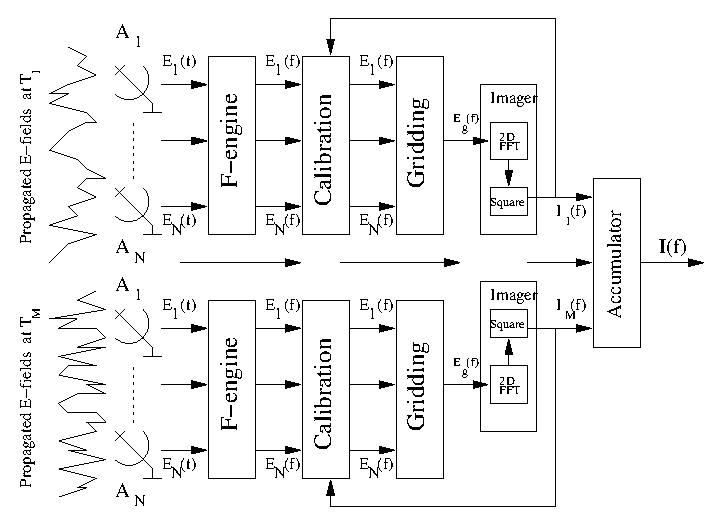
\includegraphics[width=\columnwidth]{MOFF_flowchart.eps}
  \caption{A flowchart of MOFF imaging in EPIC. The propagated electric fields shown on the left are measured as time-series $E_1(t)\ldots E_\textrm{N}(t)$ by the antennas which are then Fourier transformed by the F-engine to produce electric field spectra $E_1(f)\ldots E_\textrm{N}(f)$. They are calibrated and gridded. The gridded electric fields $E_\textrm{g}(f)$ from each time series are imaged to produce an images $I_1(f)\ldots I_\textrm{N}(f)$. These images are time-averaged to obtain the final image $I(f)$.}
  \label{fig:MOFF-flowchart}
\end{figure}

Figure~\ref{fig:FX-flowchart} shows the flowchart for software holographic imaging from a FX correlator. The antenna-based F-engine is identical to that in the MOFF processing. The electric field spectra each antenna are then cross-multiplied in the X-engine with those from all other antennas to obtain the visibilities $V_\textrm{ij}(f)$ ($\mathbf{m}(\mathbf{v})$ in matrix notation). They are calibrated and time-averaged to obtain $\langle V_\textrm{ij}(f)\rangle$ which are then gridded and imaged to obtain the image $I(f)$. The $I(f)$ obtained from both techniques are identical as explained in \S\ref{sec:math}.
\begin{figure}
  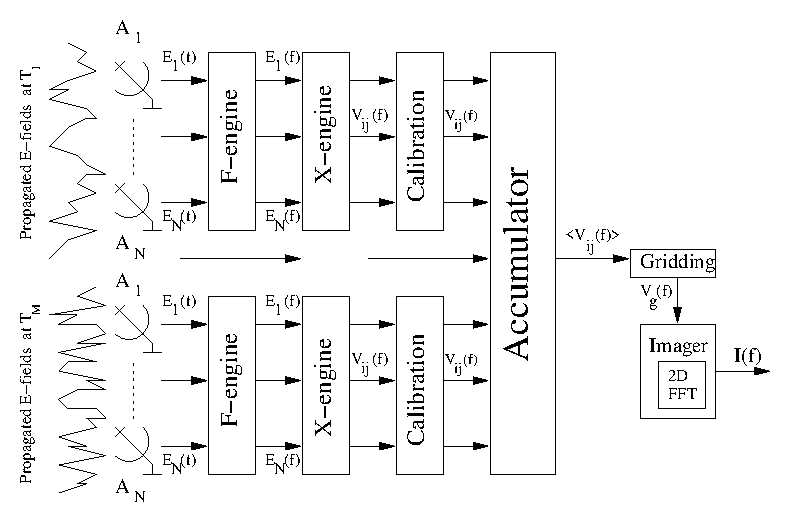
\includegraphics[width=\columnwidth]{FX_flowchart.eps}
  \caption{A flowchart of FX imaging in EPIC. The FX process flow shares the F-engine with the MOFF process. Following the F-engine, the electric fields pass through the X-engine to obtain visibilities $V_\textrm{ij}(f)$ which are calibrated and time-averaged. Then they are gridded to obtain the gridded visibilities $V_\textrm{g}(f)$ which are then imaged to obtain the image $I(f)$.}
  \label{fig:FX-flowchart}
\end{figure}

Here, we discuss the components of these architectures in detail. 

\subsection{Temporal Fourier transform}\label{sec:F-engine}

This module is common to the MOFF and FX imaging techniques. Time samples of electric fields measured by the antenna and digitized by the A/D converter is Fourier transformed to generate electric field spectra. This step can be parallelized by antennas as shown in Figure~\ref{fig:f-engine}. The output is then fed to either MOFF and FX imaging pipelines.

\begin{figure}
  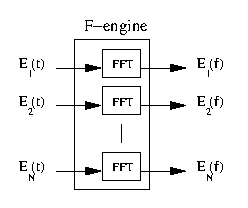
\includegraphics[width=\columnwidth]{F-engine.eps}
  \caption{Block diagram of a F-engine. The electric field data streams from antennas are Fourier transformed in parallel to generate electric field spectra.}
  \label{fig:f-engine}
\end{figure}

\subsection{Antenna-to-Grid Mapping}

A grid is generated on the coordinate system in which antenna locations are specified with a grid spacing that is at most $\lambda_\textrm{min}/2$ even at the highest frequency to ensure there is no aliasing even from regions of the sky far away from the field of view. The number of locations on the grid is restricted to be a power of 2. 

The gridding kernel in the simplest case is given by the antenna aperture illumination function, $\widetilde{B}(\mathbf{r}-\mathbf{r}_a)$, which can specified either by a functional form or as a table of values against locations around the antennas. A nearest neighbor mapping from all antenna footprints to grid locations is created using an efficient k-d tree algorithm \citep{man99}. There is no restriction here that the aperture illumination function has to be identical across antennas. 

In the most general case, this gridding kernel could contain information on the $w$-projection effect, and even other time-dependent ionospheric effects. For a stationary antenna array in the absence of any time-dependent effects, this mapping has to be determined only once in the antenna array coordinate frame. The antenna-to-grid mapping matrix, $\mathbf{M}(\mathbf{r},\mathbf{e})$ is described as a transformation matrix from the space of measured electric fields ($\mathbf{e}$) to the antenna array grid denoted by $\mathbf{r}$. Since each antenna occupies a footprint typically the size of its aperture, $\mathbf{M}(\mathbf{r},\mathbf{e})$ which is generally of size $N_\textrm{grid}\times N_\textrm{a}$, reduces to a sparse block-diagonal matrix with only $N_\textrm{a}$ blocks and roughly $N_\textrm{k}$ non-zero entries per block. Figure~\ref{fig:a2g-mapping} illustrates the antenna-to-grid mapping matrix and the grid containing the mapped aperture footprints of the antennas.

\begin{figure}
  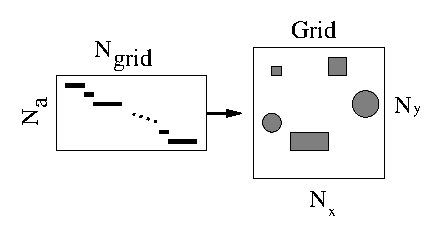
\includegraphics[width=\columnwidth]{a2g_mapping.eps}
  \caption{Block diagram of an antenna-to-grid mapping. A sparse block-diagonal matrix of total size $N_\textrm{grid}\times N_\textrm{a}$ is created where each block contains roughly the number of pixels covered by the respective kernel. The antenna aperture illumination kernels do not have to be identical to each other. A discrete set of arbitrarily placed antennas are now placed onto a regular grid.}
  \label{fig:a2g-mapping}
\end{figure}

\subsection{Calibration}

\subsection{Gridding Convolution}

The antenna array aperture illumination over the entire grid, $\widetilde{W}(\mathbf{r})$, is obtained by a projection of the individual antenna aperture illuminations:
\begin{align}
  \widetilde{W}(\mathbf{r}) &= \sum_a \widetilde{W}_a(\mathbf{r}-\mathbf{r}_a) \\
                            &= \mathbf{M}(\mathbf{r},\mathbf{e})\,\mathcal{I}(\mathbf{e}),
\end{align}
where, $\mathcal{I}(\mathbf{e})$ is a row of ones. This is achieved using efficient multiplication with the sparse matrix created in the antenna-to-grid mapping process. Unless $\widetilde{W}(\mathbf{r})$ includes time-dependent effects of the ionosphere or the instrument, it needs to be computed just once for the entire observation. However, the gridding of electric fields must be computed at every readout of the electric field spectra. Thus,
\begin{align}
  \widetilde{E}(\mathbf{r}) &= \mathbf{M}(\mathbf{r},\mathbf{e})\,E(\mathbf{e}),
\end{align}
where, $E(\mathbf{e})$ denotes the spectra of measured antenna electric fields.

In practice the grid is set to be a power of 2 such that the grid spacing is at most $\lambda/2$ even at the highest frequency in the observing band. 

\subsection{Spatial Fourier Transform}

Before the spatial Fourier transform, the gridded electric fields are padded with zeros in order to match the grid size and angular size of each image pixel that would have been obtained with software holography of output from an FX correlator. 

In MOFF imaging, these are spatially Fourier transformed followed by a squaring operation at every timestamp for every frequency channel. In FX imaging, the spatial Fourier transform is performed only once per integration timescale and does not include a squaring operation.

\subsection{Time-averaging}

In MOFF imaging, the measured antenna electric fields and the corresponding holographic electric field images are zero-mean stochastic quantities. Hence, they cannot be time-averaged to reduce noise. The statistical quantity stable with time in this case are the square of the holographic electric field images. Thus, squared images have to be formed at every instant of time before averaging as indicated in equation~\ref{eqn:dirty-image-MOFF}.

In contrast, visibilities measured by an antenna are statistically stable within an integration time interval. Hence, they are averaged after calibration as shown in equation~\ref{eqn:cc-vis}. It is advantageous to average them in visibilities before imaging because visibilities represent a compact representation of the information in images. Hence it is more computationally efficient to average antenna pair visibilities rather than images. Since this averaging has been performed already on the visibilities over an integration timescale, the imaging step has to be performed only once per integration cycle. FX imaging holds this advantage as long as the square of the number of antennas is smaller than the number of pixels on the image. 

\section{Verification}\label{sec:verify}

We use the EPIC simulator to generate electric field samples from a sky model. In our example, we use 16 frequency channels each of width $\delta f=$100~kHz, 10 point sources of random flux densities at random locations. The number of timestamps in one integration cycle was kept at four where each A/D timeseries is $1/\delta f=10\,\mu$s long. 

Show examples using simulations

Discuss PSF differences due to slight differences arising out of gridding

Apply it on LWA data

\section{Analysis and Feasibility}\label{sec:analysis}

\subsection{Scaling Relations: MOFF vs. FX}
\subsection{Scaling Up}
\subsection{Case Study}


\begin{figure}
  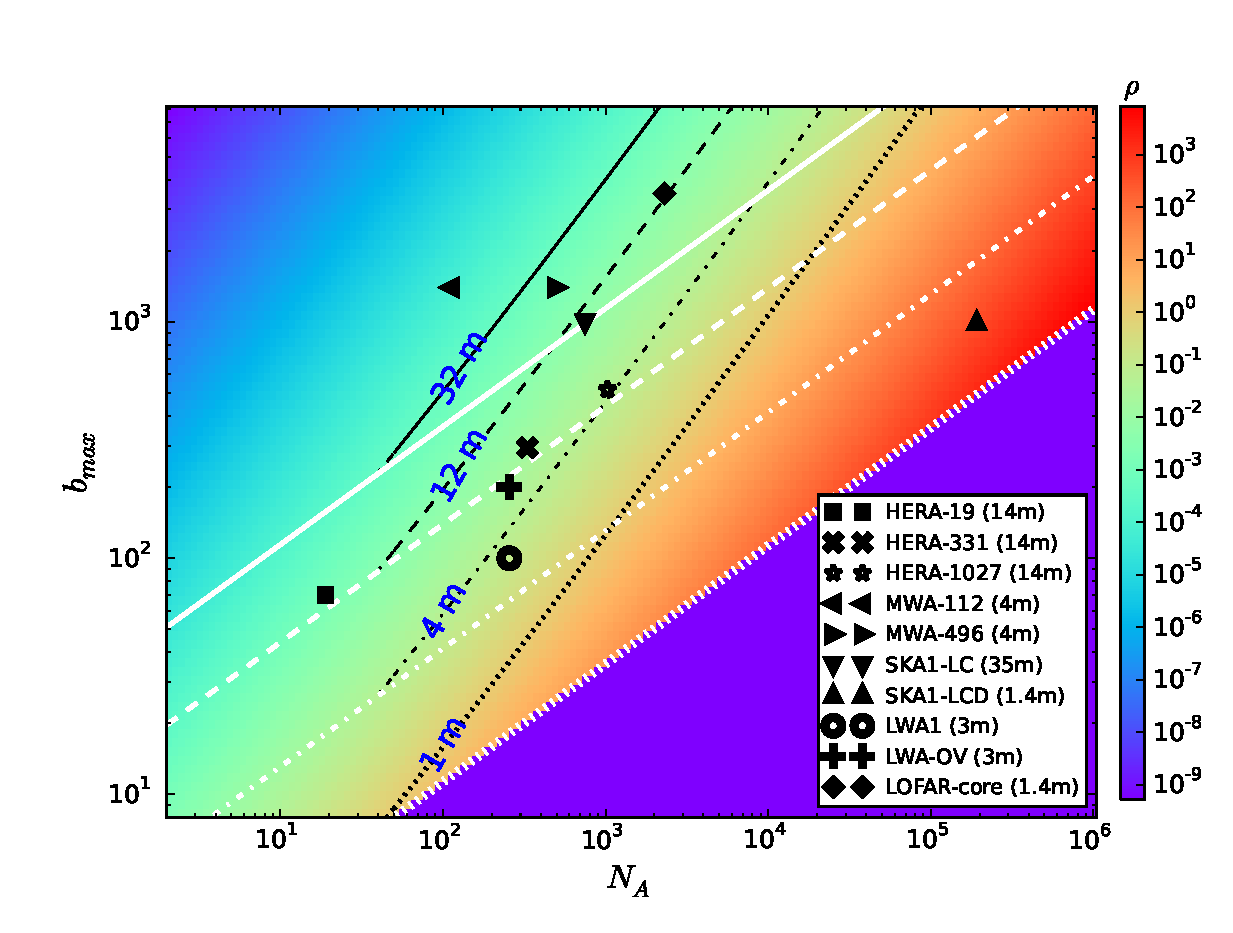
\includegraphics[width=\columnwidth]{MOFF_FX_crossover_baseline_n-antennas_rho_fov_gridding.eps}
  \caption{Current and instruments planned for future in parameter space of baseline length and number of antennas with MOFF and FX.}
  \label{fig:parameter-space-bll-nant-instruments}
\end{figure}

\begin{figure}
  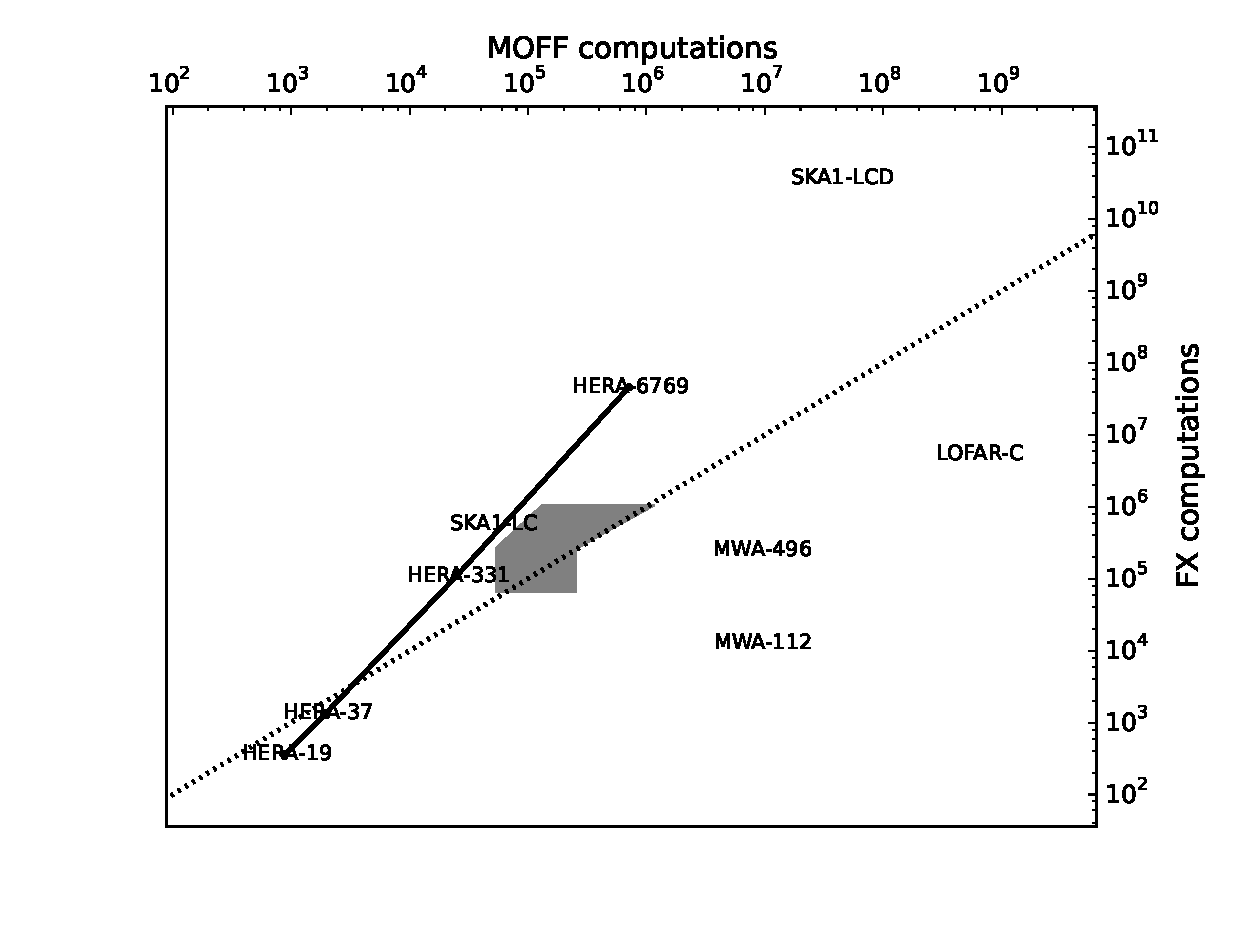
\includegraphics[width=\columnwidth]{MOFF_FX_computations_fov_gridding_annotated.eps}
  \caption{Current and instruments planned for future in parameter space of number of complex multiplies and adds with MOFF and FX.}
  \label{fig:parameter-space-computations-instruments}
\end{figure}


% \subsection{Figures and tables}

% Figures and tables should be placed at logical positions in the text. Don't
% worry about the exact layout, which will be handled by the publishers.

% Figures are referred to as e.g. Fig.~\ref{fig:example_figure}, and tables as
% e.g. Table~\ref{tab:example_table}.

% % Example figure
% \begin{figure}
% 	% To include a figure from a file named example.*
% 	% Allowable file formats are eps or ps if compiling using latex
% 	% or pdf, png, jpg if compiling using pdflatex
% 	\includegraphics[width=\columnwidth]{example}
%     \caption{This is an example figure. Captions appear below each figure.
% 	Give enough detail for the reader to understand what they're looking at,
% 	but leave detailed discussion to the main body of the text.}
%     \label{fig:example_figure}
% \end{figure}

% % Example table
% \begin{table}
% 	\centering
% 	\caption{This is an example table. Captions appear above each table.
% 	Remember to define the quantities, symbols and units used.}
% 	\label{tab:example_table}
% 	\begin{tabular}{lccr} % four columns, alignment for each
% 		\hline
% 		A & B & C & D\\
% 		\hline
% 		1 & 2 & 3 & 4\\
% 		2 & 4 & 6 & 8\\
% 		3 & 5 & 7 & 9\\
% 		\hline
% 	\end{tabular}
% \end{table}

\section{Conclusions}\label{sec:conclusions}
\section*{Acknowledgements}

The Acknowledgements section is not numbered. Here you can thank helpful
colleagues, acknowledge funding agencies, telescopes and facilities used etc.
Try to keep it short.

%%%%%%%%%%%%%%%%%%%%%%%%%%%%%%%%%%%%%%%%%%%%%%%%%%

%%%%%%%%%%%%%%%%%%%% REFERENCES %%%%%%%%%%%%%%%%%%

% The best way to enter references is to use BibTeX:

\bibliographystyle{../mnras}
\bibliography{../epic} % if your bibtex file is called example.bib


% Alternatively you could enter them by hand, like this:
% This method is tedious and prone to error if you have lots of references
% \begin{thebibliography}{99}
% \bibitem[\protect\citeauthoryear{Author}{2012}]{Author2012}
% Author A.~N., 2013, Journal of Improbable Astronomy, 1, 1
% \bibitem[\protect\citeauthoryear{Others}{2013}]{Others2013}
% Others S., 2012, Journal of Interesting Stuff, 17, 198
% \end{thebibliography}

%%%%%%%%%%%%%%%%%%%%%%%%%%%%%%%%%%%%%%%%%%%%%%%%%%

%%%%%%%%%%%%%%%%% APPENDICES %%%%%%%%%%%%%%%%%%%%%

\appendix

\section{Some extra material}

If you want to present additional material which would interrupt the flow of the main paper,
it can be placed in an Appendix which appears after the list of references.

%%%%%%%%%%%%%%%%%%%%%%%%%%%%%%%%%%%%%%%%%%%%%%%%%%


% Don't change these lines
\bsp	% typesetting comment
\label{lastpage}
\end{document}

% End of mnras_template.tex